\documentclass[12pt]{article}

\usepackage{listings}
%\lstloadlanguages{Ruby}
%\lstset{%
%basicstyle=\ttfamily\color{black},
%commentstyle = \ttfamily\color{red},
%keywordstyle=\ttfamily\color{blue},
%stringstyle=\color{orange}}
%\usepackage[dvipsnames]{xcolor}

\usepackage[utf8]{inputenc}
\usepackage[russian]{babel}
\usepackage{amsmath}
\usepackage{amssymb}
\usepackage{geometry}
\usepackage{graphicx}
\usepackage{braket}
\usepackage{hyperref}
\usepackage{esint}
\geometry{top=2cm} %поле сверху
\geometry{bottom=2cm} %поле снизу
\geometry{left=2cm} %поле справа
\geometry{right=2cm}
\usepackage{graphicx}
\usepackage{wrapfig} % Обтекание рисунков и таблиц текстом

%\newcommand{\ud}{\mathop{\mathrm{{}d}}\mathopen{}}

\begin{document}


\section*{Задачи}
\subsection*{Теория}
\begin{enumerate}
\item На рисунке - схема дорог, связывающих города А, Б, В, Г, Д, Е, Ж. По каждой дороге можно двигаться только в одном направлении, указанном стрелкой. Сколько существует различных путей из города А в город Ж?

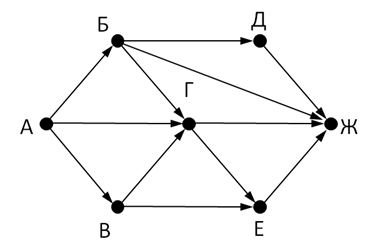
\includegraphics[width=0.3333\linewidth]{numway4}

\item Между населёнными пунктами A, B, C, D, E, F построены дороги, протяжённость которых приведена в таблице. (Отсутствие числа в таблице означает, что прямой дороги между пунктами нет). Определите длину кратчайшего маршрута из А в F.

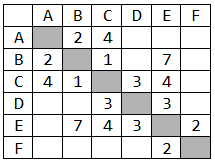
\includegraphics[width=0.3333\linewidth]{minaf}

\item На рисунке приведена весовая матрица графа. Определите, сколько рёбер имеет такой граф.

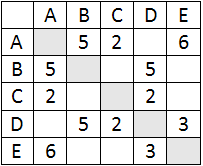
\includegraphics[width=0.3333\linewidth]{numribs1}

\end{enumerate}

\subsection*{Практика}
\begin{enumerate}
\item Вам дан текстовый файл input.txt, в котором содержатся две строки s1 и s2. Строки называются <<похожими>>, если количество букв <<a>> и <<c>> в них совпадают. Ваша задача вывести на экран, являются ли строки похожими.

\item* В текстовом файле input.txt содержится число в двоичной записи счисления. Требуется вывести на экран его десятичное представление.


\end{enumerate}

\end{document}
